\section{Introduction}
%%%%%
% should define: decision, action, context, knowledge
%%%%%

Adaptive systems have proven their suitability to handle the increasing complexity of system and their ever-changing environment.
To do so, they make adaptation decisions, in the form of actions, based on high-level policies. 
For instance, the OpenStack Watcher project~\cite{OpenStack:Watcher:Wiki} implements a MAPE-k loop to assist cloud administrators in their activities to tune and rebalance their cloud resources according to some optimization goals (e.g., CPU and network bandwidth). 
For readability purpose, we refer to adaptation decision as decision in the remaining part of this document.

Despite the reactivity of adaptation processes, impacts of their decisions can be measurable long after they have been taken.
We identified two problematics caused by this difference of paces:
\begin{itemize}
	\item How to reason over unfinished actions and their expected effects?
	\item How to diagnose the self-adaptation process?
\end{itemize}

To address them, we propose a temporal knowledge model which can trace its decisions over time, along with their circumstances and effects.
By storing them, the adaptation process could consider the ongoing actions with their expected effects.
Plus, in case of faulty decisions, developers may trace back their effects to their circumstances.

The rest of this chapter is structured as follows.
In the remaining part of this section, we motivate our approach, we summarize core concepts manipulated in adaptation processes, and we present a use case scenario based on the Luxembourg Smart Grid (\cf~Chapter~\todo{add ref}).
Then, we provide a formal definition of these concepts in Section~\ref{sec:tkm:k-formalism}.
Later, we describe the proposed data model in Section~\ref{sec:tkm:mm}.
In Section~\ref{sec:tkm:validation}, we demonstrate the applicability of our approach by applying it to the smart grid example.
We conclude this chapter in Section~\ref{sec:tkm:conclusion}.

\subsection{Motivation}

\subsubsection{Delayed action}

In this section we will motivate the need to reason over delayed actions.
To do so, we will first give four examples of these actions in.
Then we detail why the effects of actions should be considered.
Finally, we summarize and motivate the need for incorporating actions and their effect in the knowledge. 

\paragraph{Delayed action examples}
Until here, we claim that adaptation process should handle delayed actions.
In order to show their existence, we will give four different examples: two from our use case, one from cloud infrastructures and one from smart homes.
From our understanding, three phenomena can explain this delay: the time to execute the action (\cf Example 1), the time for the system to handle the new configuration (\cf Example 3) and the inertia of the measured element (\cf Example 2 and 4).

\subparagraph{Example 1: Modification of fuse states in smart grids}
Even if the Luxembourg power grid is moving to an autonomous one, not all the elements can be remotely controlled.
One example is the fuses, they still need to me open or close by a human.
In this document, open and close actions in the smart grid imply technicians who are contacted, drive to fuses places and manually change fuse states.
If several fuses need to be changed, one technician may have to drive to them, sequentially, and executes the modifications.
For example, in our case our industrial partner asks us to consider that each fuse modification should take in average 15 min whereas any incident should be detected in the minute.
Let's imagine that an incident is detected at 4p.m. and can be solved by modifying three fuses.
Before the incident will be marked as resolved, $15min * 3 = 45min$. 
The incidents will be seen as resolved by the adaptation process at 4:45p.m.
In summary, the delay of the action is due to the execution time that is not immediate.

\subparagraph[Example 2: Reduction of amps limits in smart grids]{Example 2: Reduction of amps limit in smart grids\footnote{This example is based on randomly generated data. As this action is not yet available on the Luxembourg smart grid, we miss real data. However, it reflects an hypothesis shared with our partner.}}
\begin{figure}
	\centering
	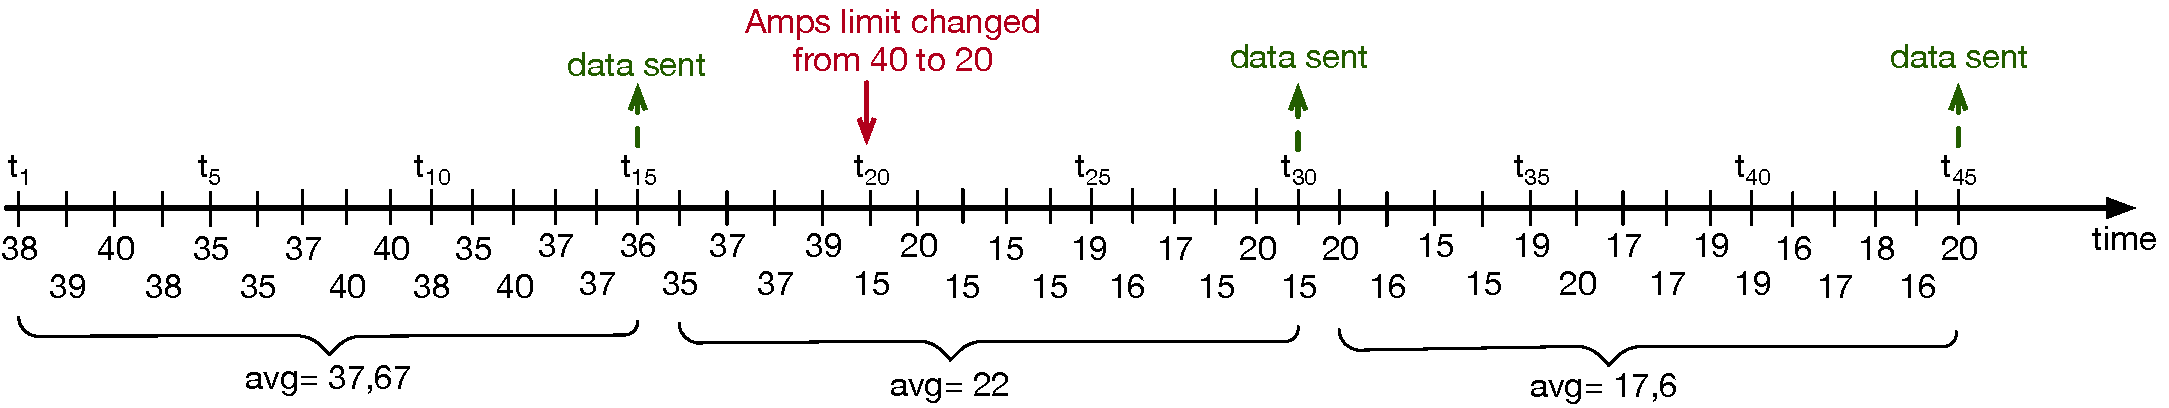
\includegraphics[width=\linewidth]{img/chapt-tkm/intro/long-action-amps-limit}
	\caption{Example of consumption measurement before and after a limitation of amps has been executed at $t_{20}$.}
	\label{fig:tkm:intro:example-long-action-amps-limit}
\end{figure}

In his smart grid project, Creos envisages controlling remotely amps limits of the grid users.
Specific plugs will be furnished to them, which will allow them managing what can be controlled and what cannot be.
One example of those is plugs to load electric vehicles.
However, due to how power consumption is measured by meters, and even if the action is near instant, the impacts of the action would not be visible immediately.
Indeed, data received by Creos corresponds to the total energy consumed since the installation.
From this information, only the average of consumed data for the last period can be computed.

In Figure~\ref{fig:tkm:intro:example-long-action-amps-limit}, we depict a scenario that shows the delay between the action is executed and the impacts are measured.
Each timepoint represents one minute, with the consumption at this moment.

Let's imagine a customer who has his or her limit set to 40 amps\footnote{It means that the user cannot consume more than 40 amps at a precise time $t_i$.} and consume near this limit.
We consider that data are sent every 15 min.
After receiving data sent at $t_{15}$ and processing them, the adaptation process detects an overload and decides to reduce the limits to 20 amps for the customer.
However, considering the delay for data to be collected and the one to sent data\footnote{Reminder: the smart grid is not built upon a fast network such a fiber network.}, the order is received and executed at $t_{20}$.
At $t_30$, new data consumption are sent, here equal to 22 amps.
Here there is two situations.
First, this reduction was enough to fix the overload.
Even in this idealistic scenario, the adaptation process should wait at worst 15min ($t_{30}$ - $t_{15}$) to see the resolution (without considering the communication time).
Second, this reduction was not enough - as the adaptation process considered that the consumption data will be at worst 20 amps and here it is 22.
Before seeing the incident as solved, the adaptation process should wait new data, sent at $t_{45}$.
It should wait around 30min ($t_{45} - t_{15}$) for this.

In summary, the delay of this action can be explained by the inertia in the consumption measurement.

\subparagraph{Example 3: Switching off a machine from a load balancer}
\begin{figure}
	\centering
	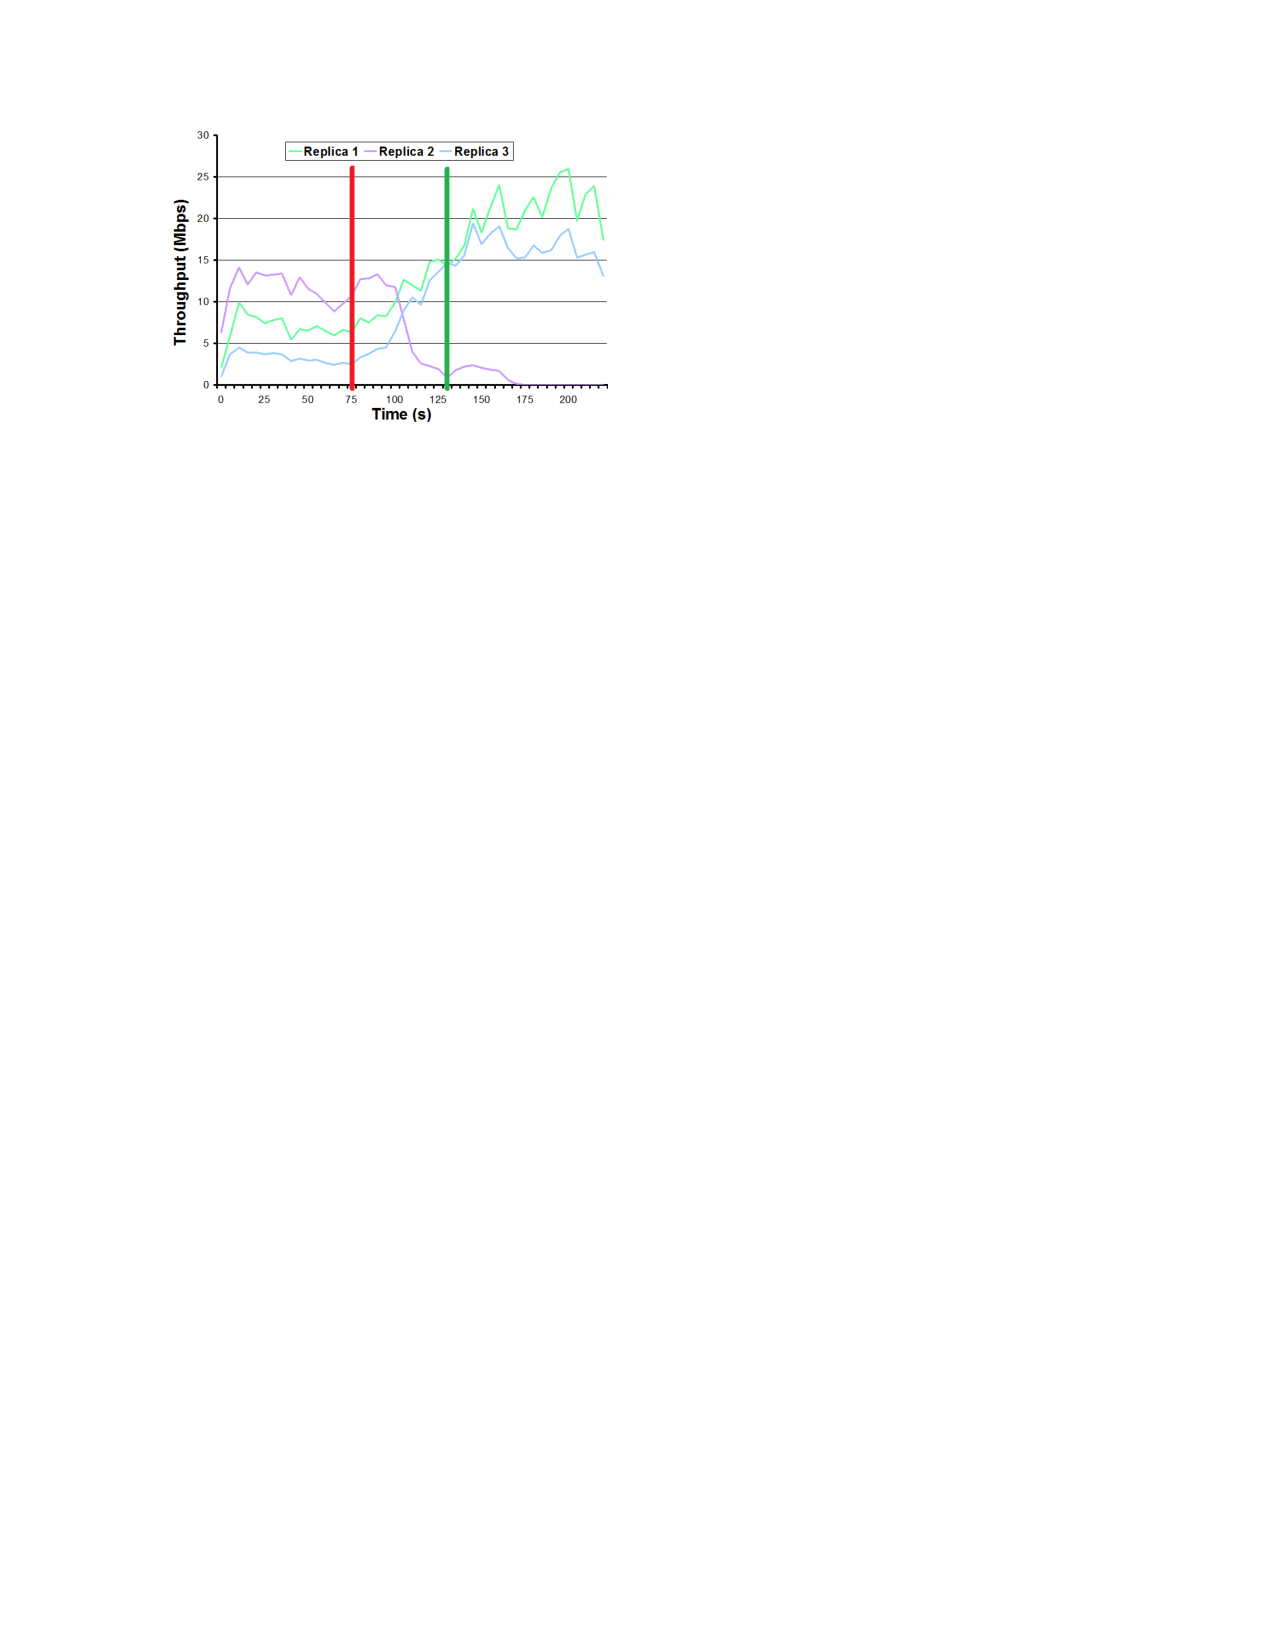
\includegraphics[width=0.5\linewidth]{img/chapt-tkm/intro/load-balencer}
	\caption{Figure extracted from~\cite{DBLP:conf/nsdi/WangBR11} that shows the delay between the time where the machine Replica 2 (R2) stop receiving new connections to prepare its disconnection (depicted by the red bar), effective around 100s later. The green bar represents the moment where the all the rules in the load balancer stop considering R2.}
	\label{fig:tkm:intro:example-load-balencer}
	
\end{figure}


An example in cloud infrastructure of long actions is to remove a machine from a load balancer, for example during a scale down operation.
Scale down operation allows cloud manager to reduce allocated resources for a specific case.
It is used either to reduce the cost of the infrastructure or to reallocate them to other tasks.
In~\cite{DBLP:conf/nsdi/WangBR11}, Wang~\etal present a load-balancing algorithm.
In their evaluation, they present the figure depicted in Figure~\ref{fig:tkm:intro:example-load-balencer} that show the evolution of the throughput after the server Replica 2 (R2) is removing from the load balancer.
The red bars shows the moment where stop receiving new connection and the green one shows the moment where it is removed from the load balancer algorithm.
However, despite these actions have been taken, R2 should finish the ongoing tasks that it is executing.
This explain why the throughout is progressively decreasing to 0 and there is a delay of around 100s between the red bars and the moment where is a no connection.

This example shows a delayed action due to the time required by the system to handle the new configuration.

\subparagraph{Example 4: Modifying home temperature through a smart home system}
Smart home systems have been implemented in order to remotely manage a house or to automatically perform routines.
For example, it allows users to close or open blinds from their smartphones from anyplace, even outside the house.
The temperature can be automatically manage by such systems, for example given targeted temperature at precise time.
However, heating or cooling a house is not immediate, it can take several hours before the targeted temperature is reached.
Plus, if the temperature sensor and the heating or cooling system or not placed nearby, the new temperature can take time before being measured.
This can be explained due to the temperature inertia plus the delay for the temperature to be propagated.


Through these four examples, we show that delayed actions can be found in different kind of systems, from CPS to cloud infrastructure.
However, not only knowing that an action is running is important but also knowing its expecting effect.
We detail this point in the next section.

\paragraph{The need to consider effects}
In the previous section we show the existence of delayed actions.
One may argue that action status is already integrated in the knowledge.
For example, the OpenStack Watcher framework stores them in a data base~\footnote{\url{https://docs.openstack.org/watcher/latest/glossary.html\#watcher-database-definition}}, accessible through an API.
However, for the best of our knowledge Watcher does not store the expecting effects of each action.
While the adaptation process knows what action is running, it does not know what it should expect from them.

Considering our example based on the modification of fuses, if the system knows that the technician is modifying fuse states, it may not know what would be the effects.
In this case, when the adaptation process analyses the system context it may wonder: what will be the next grid configuration? how the load will be balanced? will the future configuration fix all the current incidents?
If the effects are not considered by the adaptation process, then it may take suboptimal decisions.

Let's exemplify this claim through a scenario based on the modification of fuses example.
At $t_{0}$ an overload in one cable is detected and the state of three fuses need to be modified.
As explained in the previous section, this will take around 45 min.
We consider that the system can mark a incident as \textquote{being resolved}.
In the knowledge, two informations are therefore stored: the fact the the overload incident is being resolved and the fact it is done by modifying three fuses.
However, during the resolution stage, another cable is overloading.
With these informations, the system can either wait the end of the resolution of the first incident to see if both overloads will be fix or it take other actions without considering the ongoing actions.
Applying the first strategy may make the resolution of the second incident late, whereas the second one may generate suboptimal sequence of actions.
For example, the second modifications may undo what have been done before or both actions may be conflicting.

\paragraph{Conclusion}
Actions, like fuse modification in a smart grid or removing a server from a load balancer, generated during by adaptation proecess could take time upon completion. 
Moreover, the expected effects resulting from such action is reflected in the context representation only after a certain delay. 
One used workaround is the selection, often empirically, of an optimistic time interval between two iterations of the MAPE-K loop such that this interval is bigger than the longest action execution time.
However, the time to execute an action is highly influenced by system overload or failures, making such empirical tuning barely reliable.
We argue that by enriching context representation with support for past and future planned actions and their expected effects over time, we can highly enhance reasoning processes and avoid empirical tuning.

Fined and rich context information directly influences the accuracy of the actions taken.
Various techniques to represent context information have been proposed; among which we find the models@run.time~\cite{DBLP:journals/computer/MorinBJFS09, DBLP:journals/computer/BlairBF09}.
The models@run.time paradigm inherits model-driven engineering concepts to extend the use of models not only at design time but also at runtime. 
This model-based representation has proven its ability to structure complex systems and synthesize its internal state as well as its surrounding environment.

In this thesis, we propose therefore a meta-model of the knowledge which include action and their effects.
Our current approach is limited to the representation of measurable effects of any action.


\subsubsection{Diagnosis support}

Faced with growingly complex and large-scale software systems (e.g. smart grid systems), we can all agree that the presence of residual defects becomes unavoidable~\cite{DBLP:conf/icse/BarbosaLMJ17, DBLP:conf/icse/MongielloPS15, DBLP:conf/icse/HassanBB15}. 
Even with a meticulous verification or validation process, it is very likely to run into an unexpected behavior that was not foreseen at design time. Alone, existing formal modeling and verification approaches may not be sufficient to anticipate these failures~\cite{DBLP:conf/icse/TaharaOH17}. 
As such, complementary techniques need to be proposed to locate the anomalous behavior and its origin in order to handle it in a safe way.

As there might be many probable causes behind an abnormal behavior, developers usually perform a set of diagnosis routines to narrow down the scope or origin of the failure. One way to do so is by investigating the satisfaction of its requirements and the decisions that led to this system state, as well as their timing~\cite{DBLP:conf/iceccs/BencomoWSW12}.  
In this perspective, developers may set up a set of systematic questions that would help them understand why and how the system is behaving in such a way.
These questions may comprise: 
\begin{itemize}
   \item what goal(s) the system was trying to reach by executing a tactic $a$? 
   \item what were the circumstances used by a decision $d$ and its expected impact on the context?
   \item what decision(s) influenced the system's context at a time $t$? 
\end{itemize}

Bencomo~\etal~\cite{DBLP:conf/iceccs/BencomoWSW12} argue that comprehensive explanation about the system behavior contributes drastically to the quality of the diagnosis, and eases the task of troubleshooting the system behavior.
To enable this, we believe that adaptive software systems should be equipped with traceability management facilities to link the decisions made to their \textbf{(i) circumstances, that is to say, the history of the system states and the targeted requirements, and (ii) the performed actions with their impact(s) on the system}.
In particular, an \textbf{adaptive system should keep a trace of the relevant historical events}.
Additionally, it should be able to \textbf{trace the goals intended to be achieved by the system to the adaptations and the decisions that have been made, and vice versa}. 
Finally, in order to enable developers to interact with the system in a clear and understandable way, appropriate abstraction to \textbf{enable the navigation of the traces and their history should also be provided}.
Unfortunately, suitable solutions to support these features are under-investigated. 

Existing approaches~\cite{hassel13,heinrich14,ehlers11,DBLP:conf/icse/MendoncaAR14,DBLP:conf/icse/CasanovaGSA14,DBLP:conf/icse/IftikharW14a} are accompanied by built-in monitoring rules and do not allow to interact with the underlying system in a simple way. 
Moreover, they do not keep track of historical changes as well as causal relationships linking requirements to their corresponding adaptations. Only flat execution logs are stored. 

In this document, we propose a framework to structure and store the state and behavior of a running adaptive system, together with a high-level API to efficiently perform diagnosis routines. 
Our framework relies on a temporal model-based solution that efficiently abstracts decisions and their corresponding circumstances.
Specifically, based on existing approaches for modeling and monitoring adaptation processes, we identify a set of properties that characterize context, requirements, and actions in self-adaptive systems.    
Then, we formalize the common core concepts implied in adaptation processes, also referred to as knowledge, by means of temporal graphs and a set of relations that trace decisions impact to circumstances.
Finally, thanks to exposing common interfaces in adaptive processes, existing approaches in requirements and goal modeling engineering can be easily integrated into our framework. 

\subsection{Background}
Before formalizing and modeling decisions and their circumstances, we abstract common concepts implied in an adaptation process. We refer to these concepts as the knowledge.

\subsubsection{General concepts of adaptation process}

Similar to the definition provided by Kephart~\cite{DBLP:journals/computer/KephartC03}, IBM  defines adaptive systems as ``a computing environment with the ability to manage itself and \textbf{dynamically adapt} to change in accordance with \textbf{business policies and objectives}. [These systems] can perform such activities based on \textbf{situations they observe or sense in the IT environment} [...]"~\cite{computing2006architectural}.

Based on this definition, we can identify three principal concepts involved in adaptation processes.
The first concept is  \textit{actions}. They are executed in order to perform a dynamic adaptation through actuators.
The second concept is \textbf{business policies and objectives}, which is also referred to as the \textbf{system requirements} in the domain of (self-)adaptive systems.
The last concept is the observed or sensed \textbf{situation}, also known as the \textbf{context}.
The following subsections provide more details about these concepts.

\subsubsection{Context}

In this thesis, we use the widely accepted definition of context provided by Dey~\cite{DBLP:journals/puc/Dey01}: \textquote{Context is \textbf{any information that can be used to characterize} the situation of an entity. An entity is a person, place, or object that is considered relevant to the interaction between a user and [the system], including the user and [the system] themselves}.
In this section, we list the characteristics of this information based on several works found in the literature~\cite{DBLP:conf/pervasive/HenricksenIR02, chong2007context, DBLP:conf/seke/0001FNMKT14, bettini2010survey, DBLP:journals/comsur/PereraZCG14}.
We use them to drive our design choices of our Knowledge meta-model (cf. Section~\todo{Add ref}).

\paragraph{Volatility}
Data can be either \textbf{static} or \textbf{dynamic}.
Static data, also called frozen, are data that will not be modified, over time, after their creation~\cite{DBLP:conf/pervasive/HenricksenIR02, DBLP:journals/comsur/MakrisSS13, bettini2010survey, chong2007context}.
For example, the location of a machine, the first name or birth date of a user can be identified as static data. 
Dynamic data, also referred to as volatile data, are data that will be modified over time.

\paragraph{Temporality}
In dynamic data, sometimes we may be interested not only in storing the latest value, but also the previous ones~\cite{DBLP:conf/seke/0001FNMKT14, DBLP:conf/pervasive/HenricksenIR02, chong2007context}. 
We refer to these data as \textbf{historical} data.
Temporal data is not only about past values, but also future ones. 
Two kinds of future values can be identified, \textbf{predicted} and \textbf{planned}.  
Thanks to machine learning or statistical methods, dynamic data values can be \textbf{predicted}. 
\textbf{Planned} data are set by a system or a human to specify planned modification on the data.

\paragraph{Uncertainty}
One of the recurrent problems facing context-aware applications is the data uncertainty~\cite{DBLP:conf/dagstuhl/LemosGMSALSTVVWBBBBCDDEGGGGIKKLMMMMMNPPSSSSTWW10, DBLP:conf/pervasive/HenricksenIR02, DBLP:journals/comsur/MakrisSS13, bettini2010survey}.
Uncertain data are not likely to represent the reality. They contain a noise that makes it deviate from its original value.
This noise is mainly due to the inaccuracy and imprecision of sensors.
Another source of uncertainty is the behavior of the environment, which can be unpredictable.
All the computations that use uncertain data are also uncertain by propagation.

\paragraph{Source}
According to the literature, data sources are grouped into two main categories, either sensed (measured) data or computed (derived) data~\cite{DBLP:journals/comsur/PereraZCG14, chong2007context}.
%We refine this with an additional category called profiled.
%Profiled data may be set either by a user (\textbf{profiled by a human}) or by an external system (\textbf{profiled by an external}).

\paragraph{Connection}
Context data entities are usually linked using three kinds of connections: conceptual, computational, and consistency~\cite{DBLP:conf/pervasive/HenricksenIR02, bettini2010survey}.
The conceptual connection relates to  (direct) relationships between entities in the real world (e.g. smart meter and concentrator).
The computational connection is set up when the state of an entity can be linked to another one by a computation process (derived, predicted). 
Finally, the consistency connection relates entities that should have consistent values. For instance, temperature sensors belonging to the same geographical area.

\subsubsection{Requirement}
\label{sec:adaptation-req}

Adaptation processes aim at modifying the system state to reach an optimal one.
All along this process, the system should respect the \textbf{system requirements} established ahead. 
Through this paper, we use the definition provided by IEEE~\cite{iso2017systems}: ``(1) Statement that translates or expresses a need and its associated \textbf{constraints} and \textbf{conditions}, (2) \textbf{Condition or capability that must be met or possessed} by a system [...] to satisfy an agreement, standard, specification, or other formally imposed documents".\looseness=-1

Although in the literature, requirements are categorized as functional or non-functional, in this paper we use a more elaborate taxonomy introduced by Glinz~\cite{DBLP:conf/re/Glinz07}.
It classifies requirements in four categories: functional, performance, specific quality, and constraint.
All these categories share a common feature: they are all temporal.
During the life-cycle of an adaptive system, the developer can update, add or remove some requirements~\cite{DBLP:conf/icse/ChengA07, pandey2010effective}.

\subsubsection{Action}
In the IEEE Standards~\cite{iso2017systems}, an action is defined as: \textquote{\textbf{process of transformation} that \textbf{operates upon data} or other types of inputs to create data, produce outputs, or \textbf{change the state} or condition of the subject software}.

Back to adaptive systems, we can define an action as a process that, given the context and requirements as input, adjusts the system behavior.
This modification will then create new data that correspond to an output context. In the remainder of this paper, we refer to output context as impacted context, or simply impact(s).
Whereas requirements are used to add preconditions to the actions, context information is used to drive the modifications.
Actions execution have a start time and a finish time. They can either succeed, fail, or be canceled by an internal or external actor.


\subsection{Use case scenario}